\question{9.23}{
    Een autofabriek heeft een nieuw mode, de XGT, op de markt gebracht.
    In de folder staat dat het benzinegebruik laag is, namelijk gemiddeld hoogstens $7$ liter voor $100$ kilometer op de buitenweg.
    Om deze bewering te controleren, werden met zestien XGT's proefritten gemaakt van $100$ kilometer.
    Voor deze zestien proefritten werd een gemiddeld verbruik van $7,32$ liter gevonden.
    Wegens verschillen in rijstijl en rijomstandigheden mag worden aangenomen dat het benzineverbruik per $100$ kilometer wordt beschreven door een kansvariabele $X$ die normaal verdeeld is met $\sigma=0,5$ liter.
}
\begin{enumerate}[label=(\alph*)]
    \item Toets (volgens de gebruikelijke procedure) of de bewering van de fabrikant staande kan worden gehouden op basis van de uitkomsten van de proefritten (kies $\alpha=0,05$).
    \answer{
        In deze hypothesetoets geldt dat de nulhypothese $H_0: \mu \le 7$ (gemiddeld hoogstens $7$ liter per $100$ km) getest wordt tegen de alternatieve hypothese $H_1: \mu > 7$ (gemiddeld meer dan $7$ liter per $100$ km).
        In acht weken wordt het aantal klachten geteld, oftewel $n=8$
        Het geobserveerde steekproefgemiddelde is gelijk aan $\overline{x} = 7,32$ liter per $100$ km, op basis van een steekproef van $n=16$ proefritten.
        Verder is de standaarddeviatie $\sigma = 0,5$.

        Omdat we rechtszijdig toetsen, berekenen we de $z$-waarde als volgt
        \[
            z_{\alpha/2} = \invnorm(opp=1-\alpha) = \invnorm(opp=0,95) \approx 1,64499600
        \]

        De toetsingsgrootheid is in dit geval het (theoretische) steekproefgemiddelde $\overline{X}$.
        Uit de centrale limietstelling volgt dat $\overline{X} \sim N(\mu; \frac{\sigma}{\sqrt{n}})$.
        Onder de aanname dat $H_0$ waar is, geldt dat het gemiddelde $\mu = 7$.
        Merk op dat hoe hoger het steekproefgemiddelde, hoe waarschijnlijker dat de alternatieve hypothese waar is.

        Het kritieke gebied is dus van de vorm $[g, \infty)$, waarbij $g$ kan worden berekend als volgt:
            \begin{align*}
                g   &= \mu + z_{\alpha/2} \cdot \frac{\sigma}{\sqrt{n}} \\
                    &= 7 + 1,6449 \cdot \frac{0,5}{\sqrt{16}} \\
                    &\approx 7,2056 \\    
            \end{align*}

        Het kritieke gebied is dus gelijk aan $[7,2056, \infty)$.

        Het geobserveerde steekproefgemiddelde $\overline{x}=7,32$ ligt in het kritieke gebied, dus verwerpen we de nulhypothese $H_0$.
        Er is voldoende reden om aan te nemen dat het gemiddelde verbruik meer dan $7$ liter per $100$ km is, en dat de bewering in de folder niet klopt met de werkelijkheid.
    
        \begin{center}
            \resizebox{0.9\textwidth}{!}{
                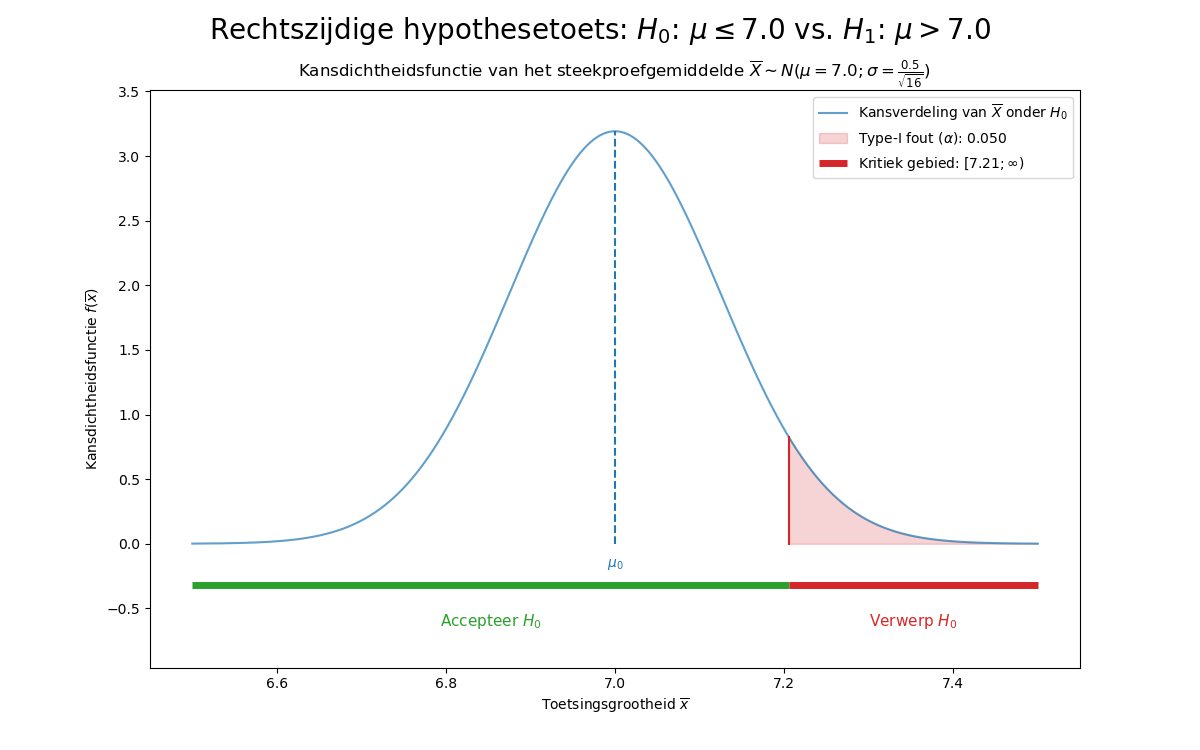
\includegraphics{opg_9.23a.png}
            }
        \end{center}
    }

    \item Bereken het onderscheidingsvermogen van de toets als in werkelijkheid zou gelden dat het gemiddeld benzineverbruik $7,30$ liter per $100$ kilometer is.
    \answer{
        Het onderscheidingsvermogen van een hypothesetoets is gelijk aan de kans $1 - \beta$ dat de nulhypothese $H_0$ wordt verworpen zodra de alternatieve hypothese $H_1$ waar is.
        In dit geval is $H_1$ waar, omdat $\mu_1=7,3$ voldoet aan $\mu > 7$.

        Stel nu dat $\mu = 7,3$.
        Dan zou gelden dat het gemiddelde benzineverbruik (in liters per $100$ km) bij 16 willekeurige proefritten $\overline{X} \sim N(\mu=7,3; \sigma = \frac{0,5}{\sqrt{16}})$. Deze kans kunnen we berekenen als de kans dat 
        Het onderscheidingsvermogen is gelijk aan de kans dat $\overline{X}$ een waarde aanneemt in het kritieke gebied dat we bij (a) hebben berekend, oftewel

        \begin{align*}
            1 - \beta   &= P(\overline{X} \ge 7,2056) \\
                        &= \normalcdf(a=7,2056; b=10^{99}; \mu=7,3; \sigma=\frac{0,5}{\sqrt{16}}) \\
                        &\approx 0,7749
        \end{align*}

        \begin{center}
            \resizebox{0.9\textwidth}{!}{
                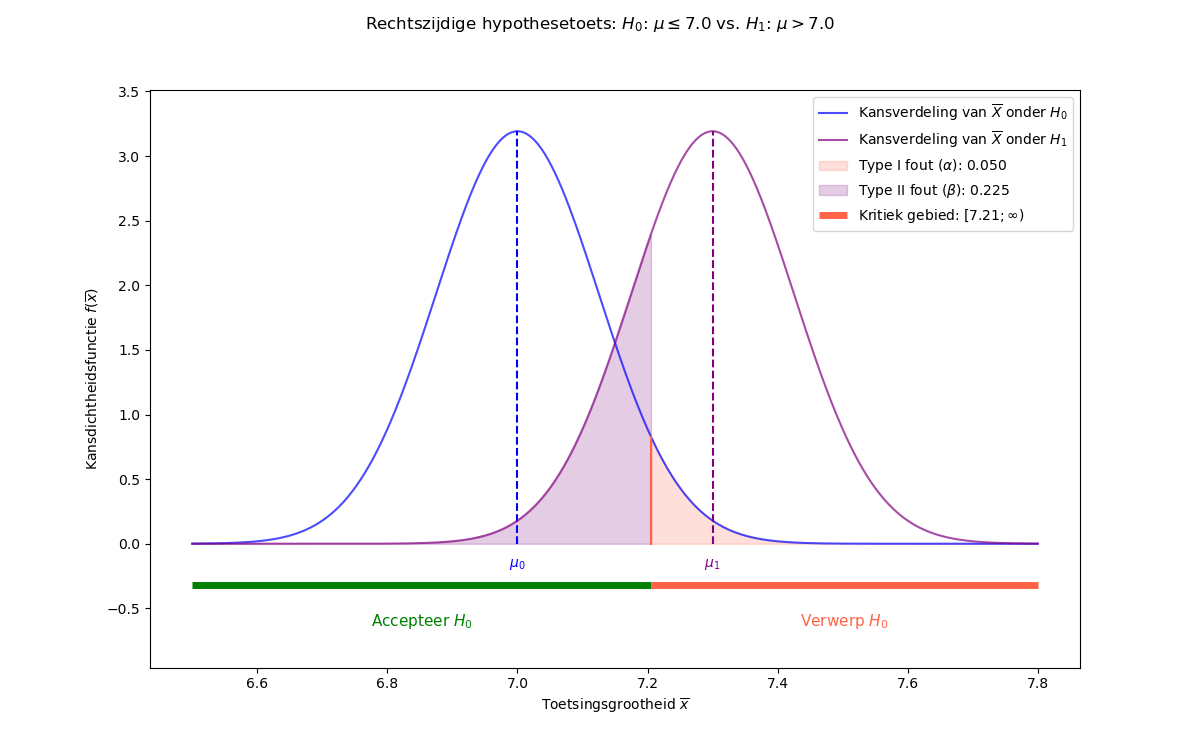
\includegraphics{opg_9.23b.png}
            }
        \end{center}
    }
\end{enumerate}